\documentclass{subfiles}

\begin{document}
	
	\section{Introduction}	
	\par In this chapter, the hyperspectral images are introduced to improve the visual output of the polygonal meshes derived from the FW LiDAR data (Chapter \ref{Visualisations}).  The combination of NERC-ARF LiDAR and hyperspectal data from New Forest (Figure \ref{fig:dataInstrumentsRelations}) for generating tree coverage maps is investigated.
	
   {\color{blue} Please note that specialised definitions (i.e. bands and level-1) are used in this chapter and if you are not familiar with these terms it is highly recommended to read Section \ref{sec:HyperspectralImages} again, which explains hyperspectral imagery.}
	
	\section{Previous Work}
	
	\par Regarding the integration of FW LiDAR and hyperspectral data in remote forest surveying, there are diverse opinions on whether the integration of multi-sensor data improves remote forest surveying. Clark et al. attempted to estimate forest biomass but no better results were observed after the integration \cite{Clark2011}, while the outcomes of Anderson et al. for observing tree species abundances structures were improved after the integration of the data \cite{Anderson2008}. 
	
	\par  Buddenbaum et al. \cite{Buddenbaum2013}, and Heinzel and Koch \cite{Heinzel2012}, used a combination of multi-sensor data for tree classifications. Buddenbaum et al. use fusion of data to generate RGB images from a combination of FW LiDAR and hyperspectral features, although the fusion reduces the dimensionality of a classifier \cite{Buddenbaum2013}. In that study, three different classifiers were implemented and the Support Vector Machines (SVMs) returned the best results. SVMs were also used in \cite{Heinzel2012} to handle the high dimensionality of the metrics (464 metrics). In that research a combination of FW LiDAR, discrete LiDAR, hyperspectral and colour infrared (CIR) images are used. Each of the 125 hyperspectral bands was directly used as a feature in the classifier, contributing to the high dimensionality. 
 
	
	
%	 Regarding tree coverage, the  Some of the FW LiDAR features are used in a digested form (i.e. the width of the waveform, which corresponds to the thickness map from Figure \ref{tab:functionalities}), and matches to the spectral signatures of each class are used to reduce the dimensionality.
	

	


	
\section{Spatial Representation of Hyperspectral Pixels for Quick Search}\label{sec:SpatialRepresentation}


	\par For the New Forest Dataset (Figure \ref{fig:dataInstrumentsRelations}), there are both FW LiDAR and hyperspectral data. {\color{blue} The data are collected from two independent instruments and, while they are flown together, each instrument has a slightly different view point, a different resolution/sensing mechanism and data collection parameters (e.g. integration time).  Therefore the data collected are not aligned to each other (e.g. for each waveform there is no trivial-correspondence to a spectral measurement).} To integrate the data geo-spatially, alignment of the data is required.  As mentioned at Section \ref{sec:HyperspectralImages}, in order to preserve the highest possible quality and reduce blurring that occurs during geo-rectification, data in the original sensing geometry (level-1) are used.
	
	\par In Anderson et al. \cite{Anderson2008}, an inverse distance weighted algorithm is used to rasterise the hyperspectral images and the pixel size is constant, 15.8m, while in this study an approach similar to Warren et al. \cite{Warren2014} is used and the resolution is changeable. The main concept of our geo-rectification algorithm is to be able to find the nearest hyperspectral pixel to a point in the fastest possible way. For that reason, a spatial representation of the hyperspectral pixels is created by importing the pixels into a 2D grid, similar to \cite{Warren2014}. The cell size of the grid in meters is constant, but the dimensions of the grid in number of squares $(n_x, n_y)$ can be varied according to the chosen average number of pixels per square $(A_{ps})$: 
	
	\begin{eqnarray}
		n_x=\sqrt{\dfrac{n_s^2}{A_{ps}}} \;\;\;\;\;\;\;\;\;\; n_y=\sqrt{\dfrac{n_l^2}{A_{ps}}}   
	\end{eqnarray} 
	
	\par Where $n_s$ is the number of samples and $n_l$ is the number of lines of the hyperspectral cube (figure \ref{fig:hyperspectralCube}).
	
	\par {\color{blue}Furthermore, Warren et al. \cite{Warren2014} uses a tree-like structure, here a structure similar to hash tables is used to spatially represent the pixels and speeding up searching. As shown in Figure \ref{fig:HashTable}, for each cell there is a bucket containing all the points that lie inside it. The hash function takes as input the unique key of the cell and returns the memory location of the corresponding bucket. The key of a cell with coordinates $(x_s,y_s)$ is is equal to $(x_s + y_s *n_x)$ where $n_x$ is the number of pixels in the x-axis.}
	
	 \begin{figure} [h!]
	 	\centering
	 	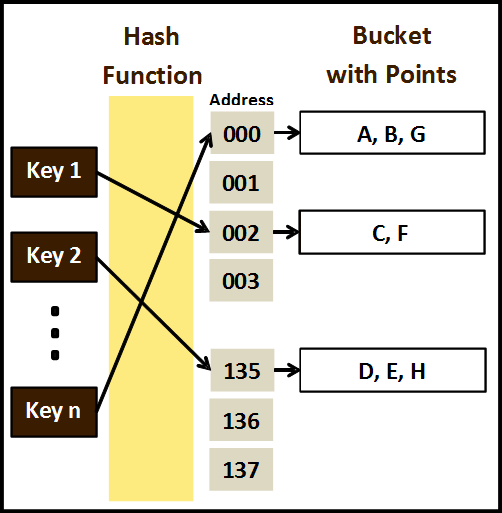
\includegraphics[width=0.55\textwidth]{img/HashTable}
	 	\caption[Hash Table]{The hash table of the spatial representation of the hyperspectral pixels; each bucket contains all the pixels in a square and has a unique key derived from the coordinates of its square. The hash function takes as input the key and returns the address in memory of the corresponding bucket. }
	 	\label{fig:HashTable}
	 \end{figure}
	
	\par The next step is for a point $(x_v, y_v, z_v)$ to find the pixel whose geolocation is the closest to it. First we project the point into 2D by dropping the $z$ coordinate and then we find the square $(x_s , y_s )$ that the projected point $\mathbf{v}(x_v , y_v)$ lies inside, as follow: 
	
    \begin{eqnarray}
	    x_s = \dfrac{x_v-X_{min}}{X_{max}-X_{min}} * n_x
    \end{eqnarray}
	
	 \begin{eqnarray}
	 x_s = \dfrac{y_v-Y_{min}}{Y_{max}-Y_{min}} * n_y 
	 \end{eqnarray}
 
	\par Where $X_{max},\; X_{min},\; Y_{max},\; Y_{min} $ are the geospatial boundaries of all the hyperspectral image and $n_x, n_x$ are the number of pixels in the x and y axis accordingly. 
	
	\par From the square $(x_s,y_s)$ we can get the set of pixels that lie inside the same square with the point of our interest. Let’s assume that the geospatial locations of these pixels are the vectors $\mathbf{g_1},\mathbf{g_2}, \mathbf{g_3}, ... , \mathbf{g_n}$ respectively. Then, by looping through that set of pixels, we can find the pixel $i$ that is most likely to be the closest pixel to the point $\mathbf{v}(x_v , y_v)$:
	\begin{eqnarray}
		i = \arg\min{|\mathbf{v}-\mathbf{g_i}|^2} .
	\end{eqnarray}
	
	\par Finally, there is the case of the closest point to be within an adjacent square and this occurs when the point is very close to the edges of the square. Even though this was not implemented in DASOS when the paper \cite{Miltiadou2015} was published, it can be done by checking the distance between the edges of the square and the point. If this distance is smaller than the distance between pixel $i$ then we can loop through the points of the corresponding adjacent square and check whether there is another pixel closer to point $\mathbf{v}$ than pixel $i$. Similarly, by checking the distance between the point $\mathbf{v}$ and the corners of the square $(x_s,y_s)$, the case of the closest point to exist inside a diagonally-adjacent square is also covered. 
	
		
\section{Projecting hyperspectral images into polygon meshes generated using FW LiDAR data}\label{sec:ProjectingHyperspectral}
	\par This section focuses on projecting the (level-1) hyperspectral images onto the polygonal meshes reconstructed from the FW LiDAR data as explained in Section \ref{sec:SurfaceReconstruction}. As shown in Figure \ref{fig:ProjectingHyperspectral}, the result is a coloured polygon mesh. That mesh is saved into two files: 
	 \begin{itemize}
	 	\item the .obj file that contains the 3D geometry and
	 	\item the .png file that contains the 2D texture image
	 \end{itemize} 	

	
		 \begin{figure} [h!]
		 	\centering
		 	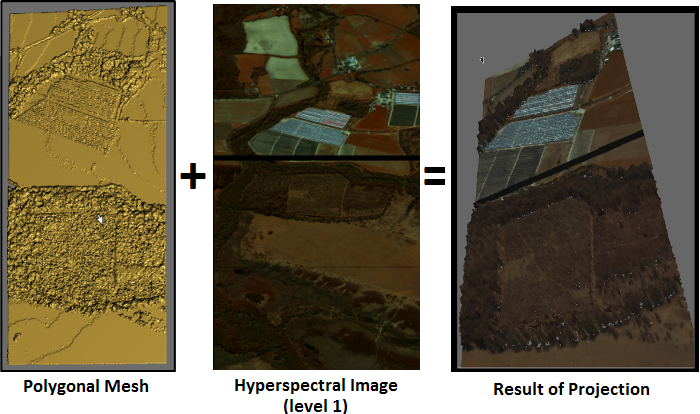
\includegraphics[width=0.9\textwidth]{img/ProjectingHyperspectral}
		 	\caption{Projecting hyperspectral images into the polygonal meshes}
		 	\label{fig:ProjectingHyperspectral}
		 \end{figure}
		 

	
			
	\par  The (level-1) hyperspectral images look deformed because the pixel size is not consistent. {\color{blue} (Figure \ref{fig:ProjectingHyperspectral} shows that inconsistency).}
	 DASOS resolves this problem by adjusting the texture coordinates of the polygonal mesh according to the geolocation of the pixels. The texture coordinates $(u, v)$ of each vertex lies inside the range $[0, 1]$ and if they are multiplied by the height/width of the texture, then the position of the corresponding pixel of the texture is given. In order to calculate the texture coordinates of each vertex $(x_v, y_v, z_v)$, the spatial representation of the hyperspectral pixels (explained at Section \ref{sec:SpatialRepresentation}) is used for quickly detecting the pixel $(x_p, y_p )$, whose geolocation is the closest to a vertex. By dividing the pixel position with the number of samples $(n_s)$ and lines $(n_l)$ in the hyperspectral image, the texture coordinates $(u, v)$ of each vertex $v(x_v , y_v)$ are calculated:
		
	\begin{eqnarray}
	u=\dfrac{x_p}{n_s} \;\;\;\;\;\;\;\;\;\; v=\dfrac{y_p}{n_l}
	\end{eqnarray}
	
	\par Regarding the outputs, the texture coordinates of the polygonal mesh are added into the .obj file, while the 2D texture is simply an image generated from three user-selected bands for the RGB colours. The width of the image is equal to the number of hyperspectral samples per line while its height is equal to the number of lines.
	
	\subsection {Results}
	

		\par The results of the projection are coloured polygonal meshes. Each coloured polygonal mesh is exported into two files:
		\begin{enumerate}
			\item the .obj file contains the 3D geometry with all the information about the vertices, edges, faces, normals and texture coordinates, and
			\item the .png is the 2D texture (an RGB image) and it is aligned with the texture coordinates of the polygonal mesh.
		\end{enumerate} 
		
		 \par Figure \ref{fig:AlignmentResults} shows how the visual output is affected by projecting hyperspectral data from different sensors and by changing the selected bands. 
		
			
		
		\begin{figure} [h!]
		  	\centering
		  	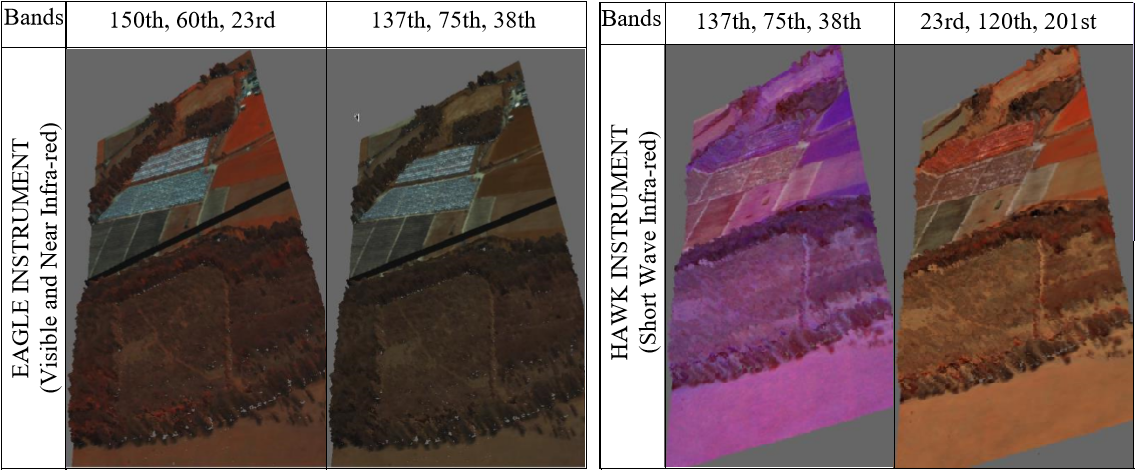
\includegraphics[width=\textwidth]{img/AlignmentEagle_Hawk}
		  	\caption[Results of Alignment]{Results of Alignment; the left table shows the results of projecting hyperspectral images from the Eagle instrument onto the polygonal meshes generated using FW LiDAR data and the right hand side table shows results using the Hawk instrument.}
		  	\label{fig:AlignmentResults}
		\end{figure}
		
	\newpage	
\section{Tree Coverage Maps}

\par As mentioned before, there are diverse opinions on whether or not integration of remotely sensed data improves forest monitoring \cite{Clark2011} \cite{Anderson2008}. For that reason, a simple pixelwise classifier was implemented to test how the integration of NERC-ARF data, using metrics generated from DASOS, performs for generating tree coverage maps.  

\par The metrics generated from both hyperspectral and FW LiDAR data are 2D aligned images (Table \ref{tbl:functionalities}). In other words, the pixel $(x, y)$ has the same geospatial coordinates in every metric. Further the resolution of the metrics depends on the resolution of the 3D voxelised FW LiDAR data (Section \ref{Voxelisation}). If the dimensions of the volume are $(x, y, z)$ then the dimensions of the metrics are $(x, y)$. For the LiDAR metrics, each pixel is coloured according to the information derived from the corresponding column. Regarding the hyperspectral metrics, (level-1) data are used to preserve the highest possible quality. The method in Section \ref{sec:SpatialRepresentation} was used for finding the pixel from the hyperspectral data with the closest geospatial location to the centre of each column of the 3D voxelised FW LiDAR.

\par The metrics used for generating tree coverage maps are grouped into two categories (FW LiDAR and hyperspectral metrics):
\begin{itemize}
	\item FW LiDAR: Height (L0), Thickness (L1), Density (L2) and First Patch (L3)
	\item Hyperspectral: Mean (H0), NDVI (H1), Standard Deviation (H2) and Spectral Signature (H3)
\end{itemize}
For more descriptive information and examples of the metrics please look at Table \ref{tbl:functionalities}, where all the functionalities of DASOS are listed.  


\subsection{Testing and Results}

\par In this case, the total accuracy was increased with the integration of FW LiDAR data and hyperspectral images. A Naïve Bayesian classifier using a multi-variance Gaussian model is applied for distinguishing tree-covered areas from the ground. The main idea is for each pixel/column to find the class that is more likely to belong to Tree or Ground.  Ground truth data were hand painted using 3D models generated with DASOS and were divided into training and testing data.  There are three test cases and, for each test case, the following metrics are used:

\begin{itemize}
	\item 1st test case uses the L0-L3 metrics that are generated from the FW LiDAR data.
	\item 2nd test case uses the H0-H3 metrics that are generated from the hyperspectral imagery.
	\item 3rd test case uses L0-L3 \& H0-H3 which is a combination of metrics generated from either FW LiDAR data or hyperspectral imagery. 
\end{itemize}

\par For each test case, an error matrix is generated to indicate the accuracy of the classification results as verified against the ground truth data (Tables \ref{tab:CoverageErrorMatrix1}, \ref{tab:CoverageErrorMatrix2} and \ref{tab:CoverageErrorMatrix3}) \cite{Congalton1991}. Each row shows the number of pixels assigned to each class relative to their actual class. For example, the first row of Table \ref{tab:CoverageErrorMatrix1} shows that 130445 pixels were classified as trees, where 125375 were actual trees and the rest 5070 were ground. From the error matrices, the classification accuracy of each test case was calculated and it is presented in Table \ref{tab:CoverageResults}.

\par Figure \ref{fig:CoverageResults} depicts the coverage maps generated for each test case. Three areas are marked for comparison. In Area 1 there is low vegetation, in Area 2 there are short trees and in Area 3 warehouses. Area 1 was incorrectly classified when only the hyperspectral data were used; when the height information of the LiDAR data was included into the classifier, area 1 was correctly classified. Similarly, Area 2 was wrongly classified when using the only FW LiDAR metrics because the height of the trees was less than the average training samples. But since features from the hyperspectral data are not height dependant, the classification results of test case 1 (with hyperspectral metrics) was better at Area 2.  Area 3 seems to confuse the first two classifiers in different ways, but the combination improved the results. 

\par Finally, to demonstrate the usefulness of DASOS's polygonal meshes, the results of the tree coverage maps were projected into the polygon representations as shown in the following Figure \ref{fig:CoverageProjectedPolygon}. 

\newpage
\begin{table}[!h]
	\centering
	\begin{tabular}{c}
	 \raisebox{-\totalheight}{\adjincludegraphics[width=0.57\linewidth]{img/ErrorMetrix1.png}}
	\end{tabular}
	\caption{Error Matrix showing the pixel-wise classification results of the 1st test case that only uses hyperspectral data.}
	\label{tab:CoverageErrorMatrix1}
\end{table}

\begin{table}[!h]
	\centering
	\begin{tabular}{c}
		\raisebox{-\totalheight}{\adjincludegraphics[width=0.57\linewidth]{img/ErrorMetrix2.png}}
	\end{tabular}
	\caption{Error Matrix showing the pixel-wise classification results of the 2nd test case that only uses FW LiDAR data.}
	\label{tab:CoverageErrorMatrix2}
\end{table}

\begin{table}[!h]
	\centering
	\begin{tabular}{c}
		\raisebox{-\totalheight}{\adjincludegraphics[width=0.57\linewidth]{img/ErrorMetrix3.png}}
	\end{tabular}
	\caption{Error Matrix showing the pixel-wise classification results of the 3rd test case that uses both hyperspectral and FW LiDAR data.}
	\label{tab:CoverageErrorMatrix3}
\end{table}


\begin{table}[!h]
	\centering
\begin{tabular}{| l || c | c | c| }
	\hline		
	& \textbf{FW LiDAR} & \textbf{Hyperspectral Imagery} & \textbf{Both} \\	
	\hline			
	\hline			
	\textbf{Tree} & 73.55\% & 90.79\% & 89.52\% \\
	\hline			
	\textbf{Ground} & 97.83\% & 83.09\% & 95.48\% \\
	\hline			
	\textbf{Mean Average Precision} & 87.58\% & 86.34\% &92.97\% \\
	\hline  
\end{tabular}
	\caption{ Classification accuracy of each test case}
	\label{tab:CoverageResults}
\end{table}



\newpage
\begin{figure} [h!]
	\centering
	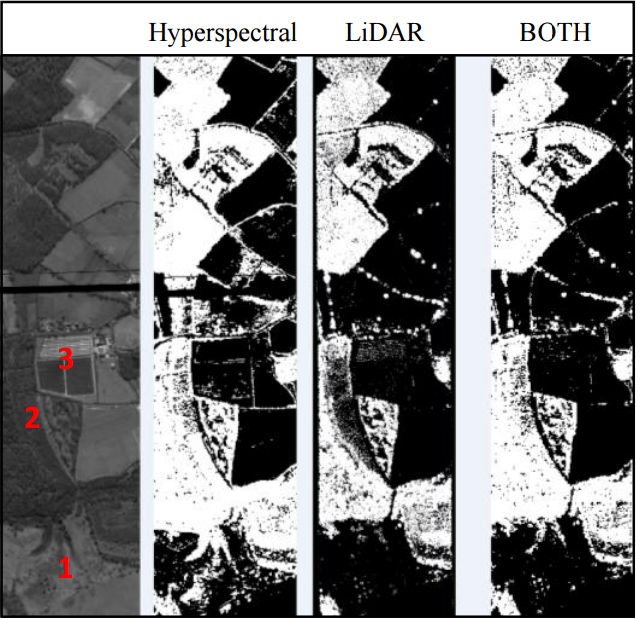
\includegraphics[width=0.7\textwidth]{img/CoverageResults}
	\caption{Visual Comparison of the results of the coverage maps }
	\label{fig:CoverageResults}
\end{figure}

\begin{figure} [h!]
	\centering
	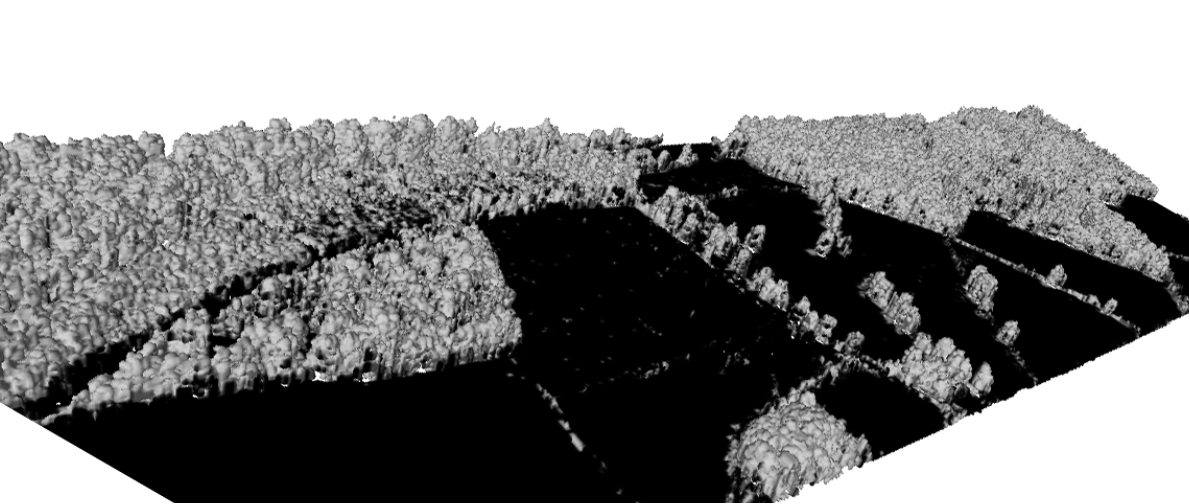
\includegraphics[width=\textwidth]{img/CoverageProjected}
	\caption[3D Coverage Model]{3D Coverage model, generated by projecting the results of the tree coverage classification into a polygonal mesh.}
	\label{fig:CoverageProjectedPolygon}
\end{figure}

\newpage\newpage
\section {Summary and Conclusions}
\par In conclusion, this chapter describes an efficient way of aligning the FW LiDAR data and hyperspectral images using a spatial representation of hyperspectral pixels. The voxelisation of the FW LiDAR data also eases the generation of aligned metrics from both datasets. Furthermore, the resolution of the metrics is changeable and depends on the user-defined resolution of the voxelised FW LiDAR data. Additionally, since the closest pixel is always selected, regardless of the distance from the point of interest, the problem of having data at different resolution is automatically resolved. 

\par Regarding the results, coloured polygonal meshes were generated using the alignment and the result demonstrated that the integration of this specific data has potential in remote forest surveying - aside from improving the visual appeal, it also improves automatic classification. This was shown using a simple classifier for generating tree coverage maps. The results were positive; the classification accuracy was improved by 5.39\% when both datasets were used.  A more sophisticated classifier would likely give even better results.



\end{document}
